\documentclass{homework}
\usepackage[utf8]{inputenc}
\usepackage{amsmath}
\usepackage{amssymb}
\usepackage{braket}
\usepackage{graphicx}

% CHANGE THE FOLLOW THREE LINES!
\newcommand{\hwname}{Vaansh Lakhwara}
\newcommand{\hwemail}{ID: 401147641}
\newcommand{\hwnum}{3}

% CHANGE THESE ONLY ONCE PER CLASS
\newcommand{\hwtype}{Assignment}
\newcommand{\hwclass}{COMP 335}

\begin{document}
\maketitle

\question

\textbf{(a)}\\
There are 10 strings of length at most 3 that are in L(r):\\
000, 1, 11, 111, 0, 00, 011, 110, 101, $\lambda$\\

\textbf{(b)}\\
There are 5 strings of length at most 3 that are not in L(r)\\
01, 10, 001, 010, 100\\

\textbf{(c)}\\
The language has number of 0's divisible by 3 or number of 1's divisible by 2.\\
Another way of saying this would be that the language has an odd number of 1's or even number of 1's.\\

\question
Let r represent a regular expression for the set of all strings on the alphabet {a, b} with no runs of length greater than 3.\\
\newline
$\therefore$ a valid way of writing r would be:\\
r = ($\lambda$ + b+bb+bbb)((a+aa+aaa)(b+bb+bbb))$^*$($\lambda$ + a+aa+aaa)\\

\question
Simplifying the given NFA we get:
\begin{center}
    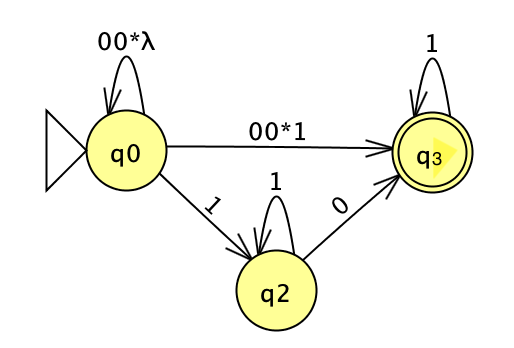
\includegraphics{A3_3.png}\\
    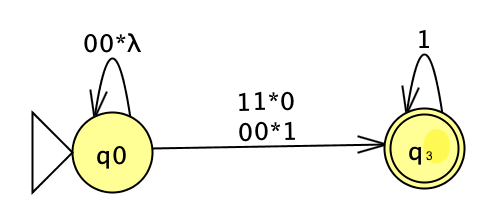
\includegraphics{A3_2.png}\\
\end{center}
From the above diagram we can infer the regular expression r to be represented as:\\
r = (00$^*$)$^*$(11$^*$0+00$^*$1)(1)$^*$\\
\question
The left side of the diagram represents: (a$^*$b+b$^*&$a)\\
The left side of the diagram represents: ((ab)$^*$+(ba)$^*$)$^*$\\
Together they form: (a$^*$b + b$^*&$a)((ab)$^*$+(ba)$^*$)$^*$\\
\begin{center}
    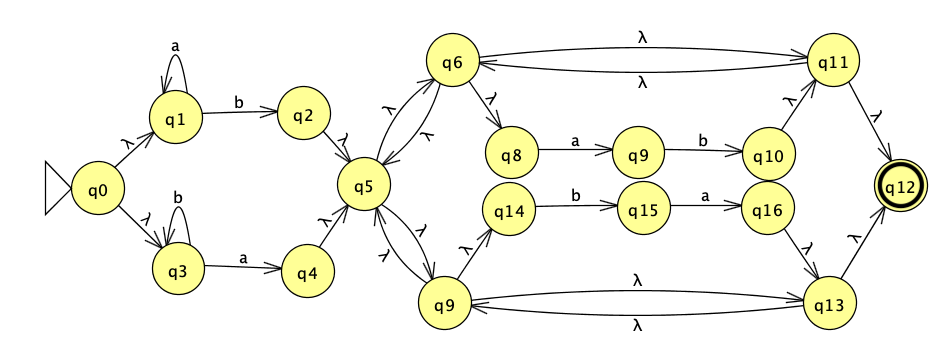
\includegraphics{A3.png}\\
\end{center}
\end{document}